\documentclass[a4paper]{article}

\usepackage[margin = 3cm]{geometry}
\usepackage{amsmath, amssymb}
\usepackage{float}
\usepackage[T1]{fontenc}
\usepackage{graphicx}
\usepackage{listings}
\usepackage{xcolor}

\lstset{%
    %backgroundcolor=\color{yellow!20},%
    basicstyle=\ttfamily%
    }%
    
\newcommand{\boldn}{\boldsymbol{n}}

\begin{document}
 
\title{VEMLAB User Guide}
\author{Massimo Frittelli}

\maketitle

\section*{Introduction}
VEMLAB is an object-oriented MATLAB library for the computation of the VEM matrices of lowest order ($k=1$) of the PDE problem
\begin{equation}
\frac{\partial u}{\partial t} - \Delta u + u = 0,
\end{equation}
in 2D and 3D, on quite general polygonal/polyhedral meshes. The library relies on the following assumptions on the mesh:
\begin{itemize}
\item in 2D, every (polygonal) element is star-shaped w.r.t. at least one point.
\item in 3D, every (polyhedral) element is star-shaped w.r.t. at least one point and so are all of its faces.
\end{itemize}

\section{The class \texttt{element2d}}
The class \texttt{element2d} represents a polygonal element in 2D with \texttt{NVert} vertexes that is star-shaped w.r.t. at least one point. To create an instance of the class, use the following constructor

\begin{lstlisting}
	obj = element2d(P, P0);
\end{lstlisting}
%
where
\begin{itemize}
\item \texttt{P} is a $\texttt{NVert} \times 3$ matrix whose rows are the coordinates of the ordered vertexes. 
\item \texttt{P0}, of size $1\times 3$, is a point w.r.t. which the element is star-shaped.
\end{itemize}

\noindent
Upon initialisation, the object stores \texttt{P} and \texttt{P0} and automatically computes several other \texttt{properties} of the element:

\begin{lstlisting}
	properties(SetAccess = private)
		P(:,3) double
		P0(1,3) double 
		NVert(1,1) double
		Area(1,1) double 
		OrientedArea(1,3) double
		Centroid (1,3) double
		Diameter(1,1) double
		K(:,:) double
		M(:,:) double
	end
\end{lstlisting}

\noindent
that can be queried from the object. In the above:
\begin{itemize}
\item \texttt{NVert} is the number of vertexes
\item \texttt{Area} is the surface area of the element
\item \texttt{OrientedArea} is a vector orthogonal to the element whose modulus is the element area
\item \texttt{Centroid} is the centroid of the element
\item \texttt{Diameter} is the diameter of the element
\item \texttt{K} is the local stiffness matrix
\item \texttt{M} is the local mass matrix
\end{itemize}

\noindent
The usage of \texttt{element2d} will be demonstrated later on.

\section{The class \texttt{element3d}}
The class \texttt{element3d} represents a polygonal element in 3D with \texttt{NVert} vertexes that is star-shaped w.r.t. at least one point and whose faces fulfill the same property.  To create an instance of the class, use the following constructor

\begin{lstlisting}
	obj = element3d(Faces, P, P0);
\end{lstlisting}
%
where 
\begin{itemize}
\item \texttt{Faces} is a $\texttt{NFaces} \times 1$ array of \texttt{element2d} representing the faces
\item \texttt{P} is a $\texttt{NVert} \times 3$ matrix whose rows are the coordinates of the vertexes
\item \texttt{P0} is a point w.r.t. which the element is star-shaped.
\end{itemize}
We remark that, even if the vertexes \texttt{P} are already contained in the \texttt{Faces}, the \texttt{property} \texttt{P} is still needed to specify vertex ordering. Upon initialisation, the object stores \texttt{Faces}, \texttt{P}, and \texttt{P0} and automatically computes several other public \texttt{properties} of the element:

\begin{lstlisting}
	properties(SetAccess = private)
		Faces(:,1) element2d
		P(:,3) double
		P0(1,3) double
		NVert(1,1) double
		NFaces(1,1) double
		Volume(1,1) double
		Centroid(1,3) double
		Diameter(1,1) double
		K(:,:) double
		M(:,:) double
	end
\end{lstlisting}

\noindent
that can be queried from the object. In the above:
\begin{itemize}
\item \texttt{NVert} is the number of vertexes and \texttt{NFaces} is the number of faces
\item \texttt{Volume}, \texttt{Centroid} and \texttt{Diameter} are self-explanatory
\item \texttt{K} is the local stiffness matrix and \texttt{M} is the local mass matrix.
\end{itemize}

\noindent
The usage of \texttt{element3d} will be demonstrated later on.

\section{A worked example in 2D: the unit square}
Here we will show the usage of \texttt{element2d} to compute the local matrices of the unit square, thereby presenting the closed-form counterpart. Consider the unit square contained in the $xy$-plane:
\begin{equation}
F = \{(x,y,z) \in \mathbb{R}^3 | (x,y) \in [0,1]^2, \ z = 0\},
\end{equation}
which can be thought of as the polygon enclosed by the vertexes $(0, 0, 0)$, $(0, 1, 0)$, $(1,1, 0)$, and $(1, 0, 0)$.  Notice that node ordering affects the resulting matrices.  We start by computing the closed form of the VEM local mass and stiffness matrices of $F$ for the lowest order case $k=1$.

\noindent
As shown in \cite{hitchhikers}, the computation of the mass and stiffness matrices relies on three fundamental matrices:
\begin{itemize}
\item $B \in \mathbb{R}^{3\times\texttt{NVert}}$;
\item $D \in \mathbb{R}^{\texttt{NVert} \times 3}$;
\item $H \in\mathbb{R}^{3\times 3}$,
\end{itemize}
whose lengthy definitions we do not report here. With the above matrices in hand, the following matrices can be obtained:
\begin{itemize}
\item $G := BD \in\mathbb{R}^{3\times 3}$;
\item $\widetilde{G} := \left[\begin{array}{ccc}
0 & 0 & 0\\ 0 & 1 & 0 \\ 0 & 0 & 1
\end{array}\right] G \in\mathbb{R}^{3\times 3}$;
\item $\Pi^\nabla_* := G^{-1}B \in \mathbb{R}^{3\times\texttt{NVert}}$;
\item $\Pi^\nabla := D\Pi^\nabla_* \in \mathbb{R}^{\texttt{NVert}\times\texttt{NVert}}$.
\end{itemize}

\noindent
Finally, the local stiffness and mass matrices are given by
\begin{align}
&K = (\Pi^\nabla_*)^T \widetilde{G} \Pi^\nabla_* + (I-\Pi^\nabla)^T(I-\Pi^\nabla);\\
&M = (\Pi^\nabla_*)^T H \Pi^\nabla_* + \text{Area(F)}(I-\Pi^\nabla)^T(I-\Pi^\nabla).
\end{align}

\noindent
For the unit square $F$,  as shown in \cite{hitchhikers}, it holds that
\begin{align}
&B = \frac{1}{4}\left[\begin{array}{c c c c}
\ \ 1 & \ \ 1 & \ \ 1 & \ \ 1\\
-\sqrt{2} & \ \ \sqrt{2} & \ \ \sqrt{2} & -\sqrt{2}\\
-\sqrt{2} & -\sqrt{2} & \ \ \sqrt{2} & \ \ \sqrt{2}
\end{array}\right];\\
%
&D = \frac{1}{4}\left[\begin{array}{c c c}
4 & -\sqrt{2} & -\sqrt{2}\\
4 & \ \ \sqrt{2} & -\sqrt{2}\\
4 & \ \ \sqrt{2} & \ \ \sqrt{2}\\
4 & -\sqrt{2} & \ \ \sqrt{2}\\
\end{array}\right];\\
%
&H = \frac{1}{24}\left[\begin{array}{c c c}
24 & 0 & 0\\
0 & 1 & 0\\
0 & 0 & 1\\
\end{array}\right].
\end{align}

\noindent
It follows that
\begin{align}
G = \frac{1}{2}&\left[\begin{array}{c c c}
2 & 0 & 0\\
0 & 1 & 0\\
0 & 0 & 1\\
\end{array}\right],
\qquad 
\widetilde{G} = \frac{1}{2}\left[\begin{array}{c c c}
0 & 0 & 0\\
0 & 1 & 0\\
0 & 0 & 1\\
\end{array}\right];\\
%
\Pi^\nabla_* = \frac{1}{4}&\left[\begin{array}{c c c c}
\ \ 1 & \ \ 1 & \ \ 1 & \ \ 1\\
-2\sqrt{2} & \ \ 2\sqrt{2} & \ \ 2\sqrt{2} & -2\sqrt{2}\\
-2\sqrt{2} & -2\sqrt{2} & \ \ 2\sqrt{2} & \ \ 2\sqrt{2}
\end{array}\right];\\
%
\Pi^\nabla = \frac{1}{4}&\left[\begin{array}{c c c c}
\ \ 3 & \ \ 1 & -1 & \ \ 1\\
\ \ 1 & \ \ 3 & \ \ 1 & -1\\
-1 & \ \ 1 & \ \ 3 & \ \ 1\\
\ \ 1 & -1 & \ \ 1 & \ \ 3\\
\end{array}\right].
\end{align}
We finally obtain the local stiffness and mass matrices:
\begin{align}
\label{stiffness_2d}
K = \frac{1}{4}&\left[\begin{array}{c c c c}
\ \ 3 &  -1 & -1 &  -1\\
 -1 & \ \ 3 &  -1 & -1\\
-1 &  -1 & \ \ 3 & -1\\
 -1 & -1 & - 1 & \ \ 3\\
\end{array}\right];\\
%
\label{mass_2d}
M = \frac{1}{48}&\left[\begin{array}{c c c c}
 \ \ \ 17 & -9 & \ \ \ 13 &  -9\\
 -9 &  \ \ \ 17 &  -9 & \ \ \ 13\\
\ \ \ 13 &  -9 &  \ \ \ 17 & -9\\
 -9 & \ \ \ 13 & - 9 & \ \ \ 17\\
\end{array}\right].
\end{align}

\noindent
We now show the usage of \texttt{element2d} to compute the matrices $K$ and $M$ numerically. To this end, we need to create an object of class \texttt{element2d}. To call the constructor, we define the array \texttt{P}
\begin{lstlisting}
	P = [0 0 0; 0 1 0; 1 1 0; 1 0 0];
\end{lstlisting}
containing the vertexes of \texttt{F} and the array \texttt{P0} as
\begin{lstlisting}
	P0 = [.5 .5 0];
\end{lstlisting}
because $F$ is star-shaped w.r.t. \texttt{P0}. Notice that, since $F$ is convex,  \texttt{P0} can be chosen as any point in $F$, even a vertex. We are ready to create the object:
\begin{lstlisting}
	F = element2d(P, P0)
\end{lstlisting}
Because there is no semicolon in the above command, the following output appears in the command window:
\begin{lstlisting}
E1 = 

  element2d with properties:

               P: [4x3 double]
              P0: [0.5000 0.5000 0]
           NVert: 4
            Area: 1
    OrientedArea: [0 0 -1]
        Centroid: [0.5000 0.5000 0]
        Diameter: 1.4142
               K: [4x4 double]
               M: [4x4 double]
\end{lstlisting}

\noindent
Accidentally, the \texttt{Centroid} coincides with \texttt{P0}. By querying the stiffness and mass matrices of \texttt{F} (with \texttt{format rat} for better readability), we can see the outputs

\begin{lstlisting}
>> E1.K

ans =

       3/4        -1/4        -1/4        -1/4     
      -1/4         3/4        -1/4        -1/4     
      -1/4        -1/4         3/4        -1/4     
      -1/4        -1/4        -1/4         3/4     
      
>> E1.M

ans =

      17/48       -3/16       13/48       -3/16    
      -3/16       17/48       -3/16       13/48    
      13/48       -3/16       17/48       -3/16    
      -3/16       13/48       -3/16       17/48    
\end{lstlisting}

\noindent
which agree with \eqref{stiffness_2d}-\eqref{mass_2d}.


\section{A worked example in 3D: the unit cube}
Here we will show the usage of \texttt{element3d} to compute the local matrices of the unit cube $E = [0,1]^3$, thereby presenting the closed-form counterpart.  Because vertex ordering is reflected in the resulting matrices, we order the vertexes as follows:
\begin{equation}
\label{cube_vertex_ordering}
(0, 0,0)\ 
(0,0, 1)\ 
(0,1, 0)\ 
(0, 1,1)\ 
(1 ,0,0)\ 
(1 ,0,1)\ 
(1 ,1,0)\ 
(1 ,1,1).
\end{equation}

\noindent
We start by computing the closed form of the VEM local mass and stiffness matrices of $E$ for the lowest order case $k=1$.  As shown in \cite{hitchhikers}, the computation of the mass and stiffness matrices relies on three fundamental matrices, similarly to the 2D case:
\begin{itemize}
\item $B \in \mathbb{R}^{4\times\texttt{NVert}}$;
\item $D \in \mathbb{R}^{\texttt{NVert} \times 4}$;
\item $H \in\mathbb{R}^{4\times 4}$,
\end{itemize}
whose lengthy definitions we do not report here. With the above matrices in hand, the following matrices can be obtained:
\begin{itemize}
\item $G := BD \in\mathbb{R}^{4\times 4}$;
\item $\widetilde{G} := \left[\begin{array}{cccc}
0 & 0 & 0 & 0\\ 0 & 1 & 0 & 0\\ 0 & 0 & 1 & 0\\ 0 & 0 & 0 & 1
\end{array}\right] G \in\mathbb{R}^{4\times 4}$;
\item $\Pi^\nabla_* := G^{-1}B \in \mathbb{R}^{4\times\texttt{NVert}}$;
\item $\Pi^\nabla := D\Pi^\nabla_* \in \mathbb{R}^{\texttt{NVert}\times\texttt{NVert}}$.
\end{itemize}

\noindent
Finally, the local stiffness and mass matrices are given by
\begin{align}
&K = (\Pi^\nabla_*)^T \widetilde{G} \Pi^\nabla_* + \text{Diam}(E)(I-\Pi^\nabla)^T(I-\Pi^\nabla);\\
&M = (\Pi^\nabla_*)^T H \Pi^\nabla_* + \text{Volume(F)}(I-\Pi^\nabla)^T(I-\Pi^\nabla).
\end{align}

\noindent
For the unit cube $E$,  it is possible to show that
\begin{align}
B = \frac{1}{8\sqrt{3}}&\left[\begin{array}{c c c c c c c c}
\sqrt{3} & \sqrt{3} & \sqrt{3} & \sqrt{3} & \sqrt{3} & \sqrt{3} & \sqrt{3} & \sqrt{3}\\
-2 & -2 & -2 & -2 & \ \ 2 & \ \ 2 & \ \ 2 & \ \ 2\\
-2 & -2 & \ \ 2 & \ \ 2 & -2 & -2 & \ \ 2 & \ \ 2\\
-2 & \ \ 2 & -2 & \ \ 2 & -2 & \ \ 2 & -2 & \ \ 2\\
\end{array}\right];\\
%
D = \frac{1}{2\sqrt{3}}&\left[\begin{array}{c c c c}
2\sqrt{3} & -1 & -1 & -1\\
2\sqrt{3} & -1 & -1 & \ \ 1\\
2\sqrt{3} & -1 & \ \ 1 & -1\\
2\sqrt{3} & -1 & \ \ 1 & \ \ 1\\
2\sqrt{3} & \ \ 1 & -1 & -1\\
2\sqrt{3} & \ \ 1 & -1 & \ \ 1\\
2\sqrt{3} & \ \ 1 & \ \ 1 & -1\\
2\sqrt{3} & \ \ 1 & \ \ 1 & \ \ 1
\end{array}\right];\\
%
H = \frac{1}{36}&\left[\begin{array}{c c c c}
36 & 0 & 0 & 0\\
0 & 1 & 0 & 0\\
0 & 0 & 1 & 0\\
0 & 0 & 0 & 1
\end{array}\right].
\end{align}

\noindent
It follows that
\begin{align}
G = \frac{1}{3}&\left[\begin{array}{c c c c}
3 & 0 & 0 & 1\\
0 & 1 & 0 & 0\\
0 & 0 & 1 & 0\\
0 & 0 & 0 & 1
\end{array}\right],
\qquad 
\widetilde{G} = \frac{1}{3}\left[\begin{array}{c c c c}
0 & 0 & 0 & 1\\
0 & 1 & 0 & 0\\
0 & 0 & 1 & 0\\
0 & 0 & 0 & 1
\end{array}\right];\\
%
\Pi^\nabla_* =\frac{1}{8}&\left[\begin{array}{c c c c c c c c}
1 & 1 & 1 & 1 & 1 & 1 & 1 & 1\\
-2\sqrt{3} & -2\sqrt{3} & -2\sqrt{3} & -2\sqrt{3} & \ \ 2\sqrt{3} & \ \ 2\sqrt{3} & \ \ 2\sqrt{3} & \ \ 2\sqrt{3}\\
-2\sqrt{3} & -2\sqrt{3} & \ \ 2\sqrt{3} & \ \ 2\sqrt{3} & -2\sqrt{3} & -2\sqrt{3} & \ \ 2\sqrt{3} & \ \ 2\sqrt{3}\\
-2\sqrt{3} & \ \ 2\sqrt{3} & -2\sqrt{3} & \ \ 2\sqrt{3} & -2\sqrt{3} & \ \ 2\sqrt{3} & -2\sqrt{3} & \ \ 2\sqrt{3}\\
\end{array}\right];\\
%
\Pi^\nabla = \frac{1}{4}&\left[\begin{array}{c c c c c c c c}
2 & 1 & 1 & 0 & 1 & 0 & 0 & \!\!\!\! -1\\
1 & 2 & 0 & 1 & 0 & 1 & \!\!\!\! -1 & 0\\
1 & 0 & 2 & 1 & 0 & \!\!\!\! -1 & 1 & 0\\
0 & 1 & 1 & 2 & \!\!\!\! -1 & 0 & 0 & 1\\
1 & 0 & 0 & \!\!\!\! -1 & 2 & 1 & 1 & 0\\
0 & 1 & \!\!\!\! -1 & 0 & 1 & 2 & 0 & 1\\
0 & \!\!\!\! -1 & 1 & 0 & 1 & 0 & 2 & 1\\
\!\!\!\! -1 & 0 & 0 & 1 & 0 & 1 & 1 & 2
\end{array}\right].
\end{align}

\noindent
We finally obtain the local stiffness and mass matrices:
\begin{align}
\label{stiffness_3d}
\begin{split}
K = \frac{1}{16}&\left[\begin{array}{c c c c c c c c}
\ \  3        &   \ \     1        &  \ \      1      &       -1       &    \ \     1       &      -1      &       -1            & -3       \\
  \ \       1          &  \ \    3      &       -1       &    \ \     1     &        -1         &   \ \    1        &     -3        &     -1       \\
   \ \      1       &      -1     &    \ \       3       &    \ \     1        &     -1       &      -3        &  \ \      1      &       -1       \\
      -1     &      \ \     1      &      \ \    1      &      \ \    3       &      -3      &       -1       &      -1      &     \ \     1       \\
   \ \      1        &     -1        &     -1     &        -3       &    \ \     3       &   \ \      1        &    \ \    1       &     -1       \\
      -1       &    \ \     1       &      -3       &      -1       &   \ \      1       &    \ \     3      &       -1       &   \ \      1       \\
      -1     &        -3      &    \ \      1       &      -1      &    \ \     1       &      -1       &   \ \      3       &    \ \     1       \\
      -3       &      -1       &      -1     &     \ \      1      &       -1      &   \ \       1     &      \ \     1        &   \ \     3    
\end{array}\right]\\
+ \frac{\sqrt{3}}{4}&\left[\begin{array}{c c c c c c c c}
 \ \  2      &       -1       &      -1            &  \ \  0       &      -1      &      \ \     0      &      \ \    0             & \ \   1       \\
      -1     &        \ \    2       &    \ \      0      &      -1      &       \ \    0       &      -1        &    \ \     1              &  \ \  0       \\
      -1      &     \ \      0       &    \ \      2     &        -1      &     \ \      0       &        \ \  1       &      -1   &       \ \         0       \\
    \ \      0     &        -1        &     -1      &      \ \     2        &    \ \     1       &        \ \  0        &    \ \     0 &           -1       \\
      -1      &    \ \       0        &    \ \     0        &    \ \    1        &     \ \    2       &      -1       &      -1       &    \ \      0       \\
     \ \     0     &        -1      &      \ \     1        &   \ \      0     &       -1       &        \ \  2        &     \ \    0  &           -1       \\
     \ \     0        &    \ \     1      &       -1      &     \ \      0      &      -1       &        \ \  0       &     \ \    2  &           -1       \\
     \ \     1       &      \ \    0       &   \ \       0     &        -1       &      \ \    0       &      -1        &     -1    &      \ \       2   \\
\end{array}\right];
\end{split}\\
%
\label{mass_3d}
M = \frac{1}{96}&\left[\begin{array}{c c c c c c c c}
 \ \ 51        &    -22       &     -22        &       1       &     -22        &       1        &    \ \    1        &    \ \   24     \\  
     -22        &      \ \ 51        &      1        &    -22     &      1        &    -22            &  \ \  24      &        1       \\
     -22      &        1       &    \ \    51    &        -22      &        1      &    \ \     24           & -22       &       1       \\
       1      &      -22       &     -22      &     \ \    51        &   \ \    24        &      1             & 1       &     -22       \\
     -22    &          1        &      1       &     \ \   24     &     \ \     51       &     -22           & -22       &       1       \\
       1      &      -22        &    \ \   24      &        1      &      -22       &     \ \   51             & 1   &         -22       \\
       1          &   \ \  24     &       -22       &       1      &      -22       &       1            &  \ \ 51       &     -22       \\
    \ \    24         &     1       &       1     &       -22      &        1      &      -22           & -22      &     \ \    51 
\end{array}\right].
\end{align}

\noindent
We now show the usage of \texttt{element3d} to compute the matrices $K$ and $M$ numerically. To this end, we need to create an object of class \texttt{element3d}. To call the constructor, we first need to create six instances of \texttt{element2d} representing the faces of $E$:

\begin{lstlisting}
P1 = [0 0 0; 0 1 0; 1 1 0; 1 0 0]; % bottom face
E1 = element2d(P1, sum(P1,1)/4);

P2 = [0 0 1; 0 1 1; 1 1 1; 1 0 1]; % top face
E2 = element2d(P2, sum(P2,1)/4);

P3 = [0 0 0; 0 1 0; 0 1 1; 0 0 1]; % back face
E3 = element2d(P3, sum(P3,1)/4);

P4 = [1 0 0; 1 1 0; 1 1 1; 1 0 1]; % front face
E4 = element2d(P4, sum(P4,1)/4);

P5 = [0 0 0; 1 0 0; 1 0 1; 0 0 1]; % left face
E5 = element2d(P5, sum(P5,1)/4);

P6 = [0 1 0; 1 1 0; 1 1 1; 0 1 1]; % right face
E6 = element2d(P6, sum(P6,1)/4);
\end{lstlisting}

\noindent
For each of the faces,  we have chosen \texttt{P0} as the midpoint of its vertexes for convenience, but of course other choices are possible since every face is convex and thus star-shaped w.r.t. every point of the face itself.  We are ready to create the \texttt{element3d}:
\begin{lstlisting}
P = unique([P1; P2; P3; P4; P5; P6],`rows');
E = element3d([E1;E2;E3;E4;E5;E6], P, sum(P,1)/8);
\end{lstlisting}
We have used the command \texttt{unique} to extract a set of all vertexes with no repetitions. MATLAB will sort the vertexes in \texttt{P} in ``increasing order'', that is as in \eqref{cube_vertex_ordering}.  Again, the \texttt{P0} is chosen as the midpoint of all vertexes for convenience. Let us have a look at the 3D element \texttt{E}:
\begin{lstlisting}
>> E

E = 

  element3d with properties:

       Faces: [6x1 element2d]
           P: [8x3 double]
          P0: [0.5000 0.5000 0.5000]
       NVert: 8
      NFaces: 6
      Volume: 1.0000
    Centroid: [0.5000 0.5000 0.5000]
    Diameter: 1.7321
           K: [8x8 double]
           M: [8x8 double]
\end{lstlisting}

\noindent
By querying the stiffness and mass matrices of \texttt{E}, we can see the outputs

\begin{lstlisting}
>> format
>> E.K

ans =

    1.0535  -0.3705  -0.3705  -0.0625  -0.3705  -0.0625  -0.0625   0.2455
   -0.3705   1.0535  -0.0625  -0.3705  -0.0625  -0.3705   0.2455  -0.0625
   -0.3705  -0.0625   1.0535  -0.3705  -0.0625   0.2455  -0.3705  -0.0625
   -0.0625  -0.3705  -0.3705   1.0535   0.2455  -0.0625  -0.0625  -0.3705
   -0.3705  -0.0625  -0.0625   0.2455   1.0535  -0.3705  -0.3705  -0.0625
   -0.0625  -0.3705   0.2455  -0.0625  -0.3705   1.0535  -0.0625  -0.3705
   -0.0625   0.2455  -0.3705  -0.0625  -0.3705  -0.0625   1.0535  -0.3705
    0.2455  -0.0625  -0.0625  -0.3705  -0.0625  -0.3705  -0.3705   1.0535
      
>> format rat
>> E.M

ans =

    17/32  -11/48  -11/48    1/96  -11/48    1/96    1/96    1/4
   -11/48   17/32    1/96  -11/48    1/96  -11/48    1/4     1/96
   -11/48    1/96   17/32  -11/48    1/96    1/4   -11/48    1/96    
     1/96  -11/48  -11/48   17/32    1/4     1/96    1/96  -11/48    
   -11/48    1/96    1/96    1/4    17/32  -11/48  -11/48    1/96    
     1/96  -11/48    1/4     1/96  -11/48   17/32    1/96  -11/48    
     1/96    1/4   -11/48    1/96  -11/48    1/96   17/32  -11/48    
     1/4     1/96    1/96  -11/48    1/96  -11/48  -11/48   17/32  
\end{lstlisting}

\noindent
which agree with \eqref{stiffness_3d}-\eqref{mass_3d} up to machine precision.


\section{Numerical examples for bulk problems}

\subsection{Laplace equation on the cube}
We now test the convergence of Virtual Elements, implemented via VEMLAB,  for the following  Laplace equation on the unit cube $\Omega = [0,1]^3$:
\begin{equation}
\label{experiment_laplace_equation_3d}
\begin{cases}
-&\Delta u + u = (3\pi^2+1)\cos(\pi x)\cos(\pi y)\cos(\pi z) \qquad \text{in}\ \Omega\\
&\nabla u \cdot \boldsymbol{n} = 0 \qquad \text{on}\ \partial \Omega
\end{cases}
\end{equation}
whose exact solution  is given by
\begin{equation}
u(x,y,z) = \cos(\pi x)\cos(\pi y)\cos(\pi z).
\end{equation}
We consider a sequence of nine cubic meshes $i=1,\dots,9$. The $i$-th mesh, obtained by subdividing each dimension into $5i$ intervals,  has $(5i)^3$ elements, $N_i = (5i+1)^3$ nodes and meshsize $h_i = \sqrt{3}/(5i)$, as displayed in Table \ref{tab:laplace_3d_convergence}. On each mesh we solve the discrete problem,  we compute the error in $L^2(\Omega)$ norm and the respective convergence rate. As shown in Table \ref{tab:laplace_3d_convergence}, the convergence in $L^2(\Omega)$ norm is optimal, i.e. quadratic. The numerical solution obtained on the finest mesh is plotted in Fig.  \ref{fig:laplace_3d_numsol}.

\begin{table}[H]
\caption{Laplace equation \eqref{experiment_laplace_equation_3d} on the unit cube $\Omega = [0,1]^3$. The VEM implemented in VEMLAB shows optimal quadratic convergence in $L^2(\Omega)$ norm.}
\begin{center}
\begin{tabular}{c | c | c | c | c}
$i$ & $N$ & $h$ & $L^2(\Omega)$ error & $L^2(\Omega)$ rate\\
\hline
1 & 216 & 0.3464 &   2.1663e-02 &     -\\
2 & 1331 & 0.1732 & 1.9934e-02 & 0.1200    \\
3 & 4096 & 0.1155 & 1.0393e-02 & 1.6062    \\
4 & 9261 & 0.0866 &  6.1700e-03 & 1.8126    \\
5 &  17576 &  0.0693 & 4.0474e-03 & 1.8895    \\
6 & 29791  & 0.0577 & 2.8484e-03 & 1.9269    \\
7 &  46656 & 0.0495 & 2.1095e-03 & 1.9480    \\
8 & 68921 & 0.0433 & 1.6235e-03  & 1.9611   \\
9 & 97336 & 0.0385 &  1.2873e-03 &  1.9698
\end{tabular}
\end{center}
\label{tab:laplace_3d_convergence}
\end{table}

\begin{figure}[H]
\begin{center}
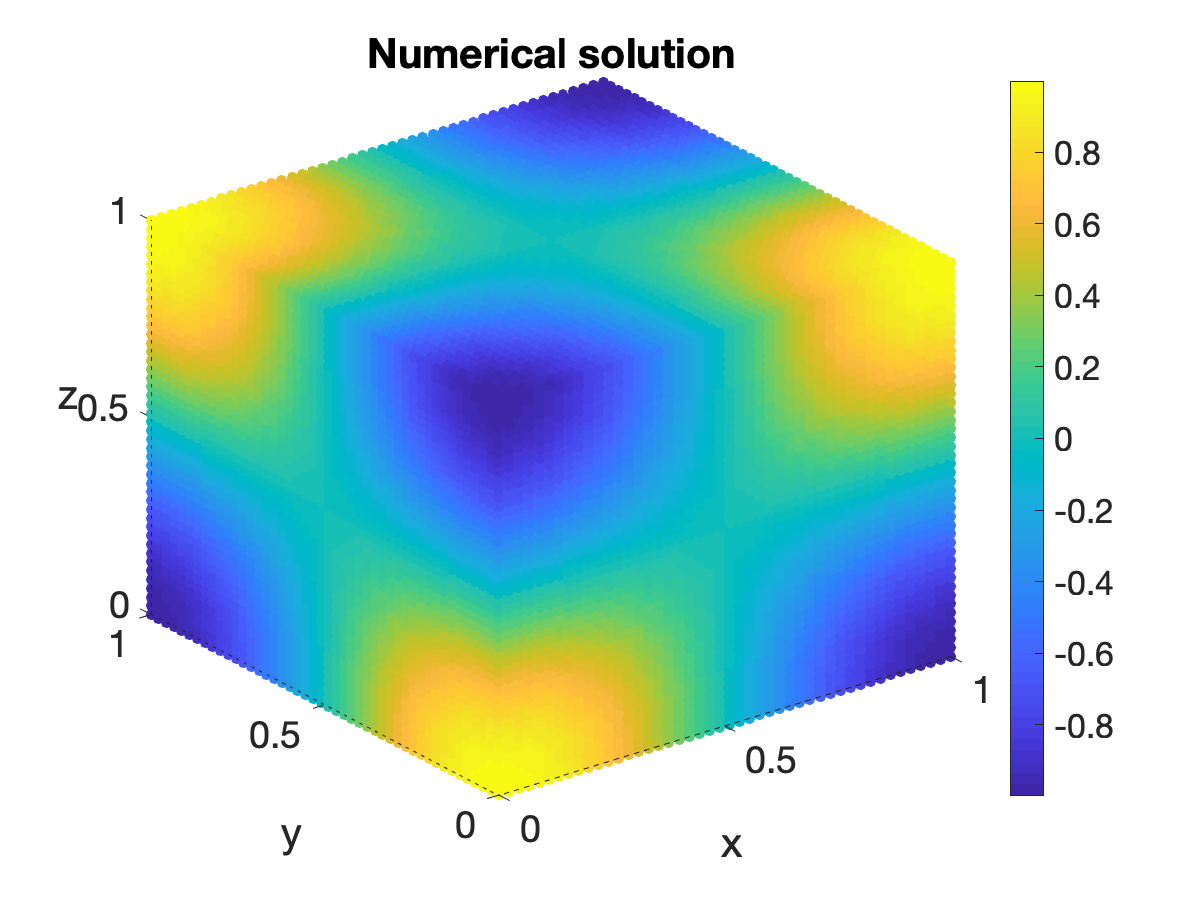
\includegraphics[scale=0.5]{laplace3dcube_numsol_Nx46.eps}
\end{center}
\caption{Laplace equation \eqref{experiment_laplace_equation_3d} on the unit cube $\Omega = [0,1]^3$: numerical solution obtained on the finest mesh for $i=9$ with $N= 97336$ nodes.}
\label{fig:laplace_3d_numsol}
\end{figure}

 
\subsection{Laplace equation on the sphere}
\label{sec:laplace_sphere}
We now consider another domain, the unit sphere $\Omega$ in 3D. The test problem, in spherical coordinates, is as follows
\begin{equation}
\label{experiment_laplace_equation_3d_sphere}
\begin{cases}
-&\Delta u + u = 4(3-5r^2) + (1-r^2)^2 \qquad \text{in}\ \Omega\\
&\nabla u \cdot \boldsymbol{n} = 0 \qquad \text{on}\ \partial \Omega
\end{cases}
\end{equation}
whose exact solution in spherical coordinates is given by
\begin{equation}
u(x,y,z) = (1-r^2)^2
\end{equation}
We consider a sequence of four cubic meshes $i=1,\dots,4$. The $i$-th mesh is obtained by subdividing each dimension into $5i$ intervals, thereby producing a cubic bounding mesh.  The cubic elements that are not fully contained in the sphere are then discarded. Finally, the outer faces of the resulting cubic mesh are extruded to fill the outer part of the sphere with irregular $8$-vertex polyhedra.  Such a mesh is shown in Fig.  \ref{fig:extruded_mesh_sphere}. On each mesh we solve the discrete problem,  we compute the error in $L^2(\Omega)$ norm and the respective convergence rate. As shown in Table \ref{tab:laplace_3d_convergence_sphere}, the convergence in $L^2(\Omega)$ norm is optimal, i.e. quadratic. The numerical solution obtained on the finest mesh is plotted in Fig.  \ref{fig:laplace_3d_numsol_sphere}.

\begin{figure}[H]
\begin{center}
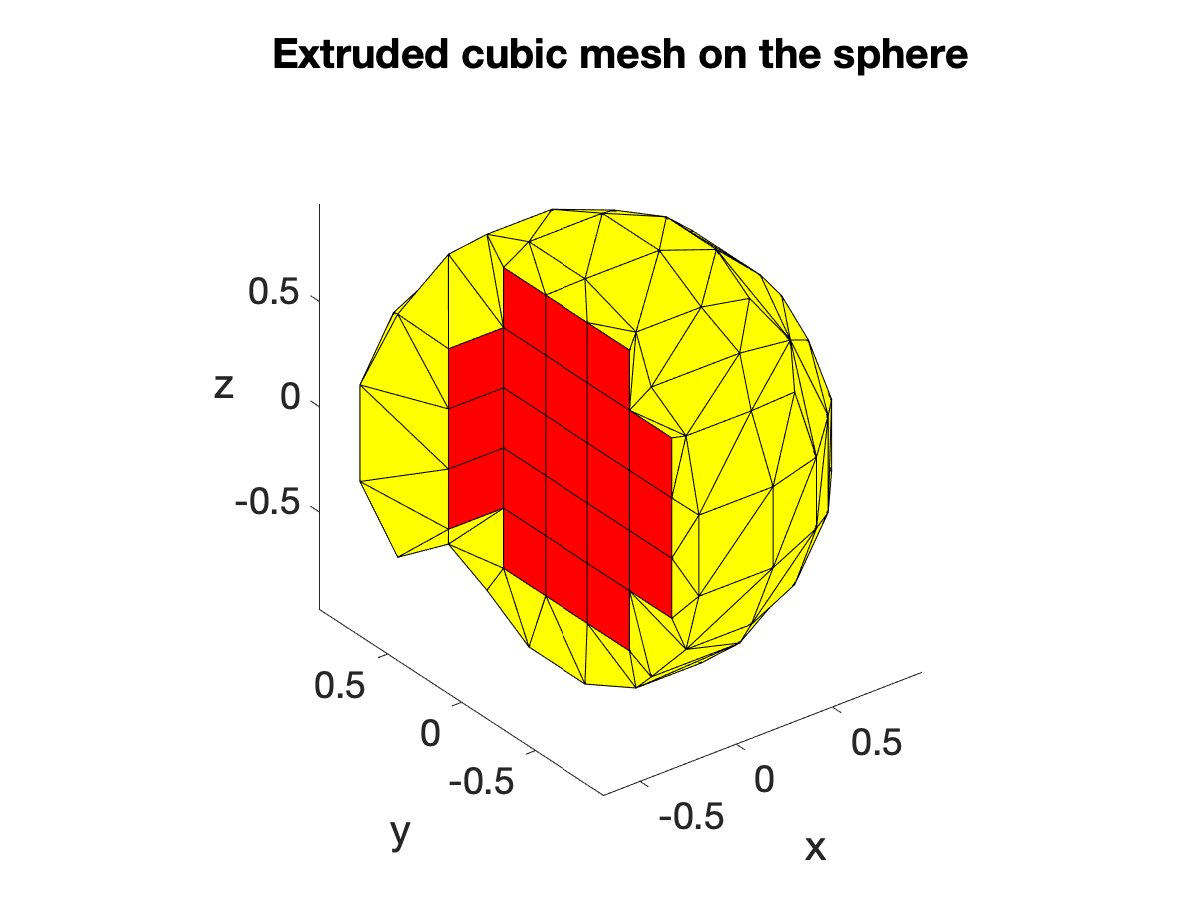
\includegraphics[scale=0.5]{extruded_mesh_sphere.eps}
\end{center}
\caption{Example of an extruded cubic mesh on the unit sphere.  The outermost elements, highlighted in yellow are irregular (but still star-shaped or even convex) $8$-vertex polyhedra.  The interior is filled with cubes (red).}
\label{fig:extruded_mesh_sphere}
\end{figure} 

\begin{table}[H]
\caption{Laplace equation \eqref{experiment_laplace_equation_3d_sphere} on the unit sphere $\Omega$ in 3D. The VEM implemented in VEMLAB shows optimal quadratic convergence in $L^2(\Omega)$ norm.}
\begin{center}
\begin{tabular}{c | c | c | c | c}
$i$ & $N$ & $h$ & $L^2(\Omega)$ error & $L^2(\Omega)$ rate\\
\hline
1 & 111 & 0.6928 &   1.3767 &  -   \\
2 & 799 & 0.3464 & 4.4137e-01 & 1.6412    \\
3 & 5749 & 0.1732 & 1.2532e-01 & 1.8164    \\
4 & 40381 & 0.0866 &  3.3139e-02 & 1.9190
\end{tabular}
\end{center}
\label{tab:laplace_3d_convergence_sphere}
\end{table}

\begin{figure}[H]
\begin{center}
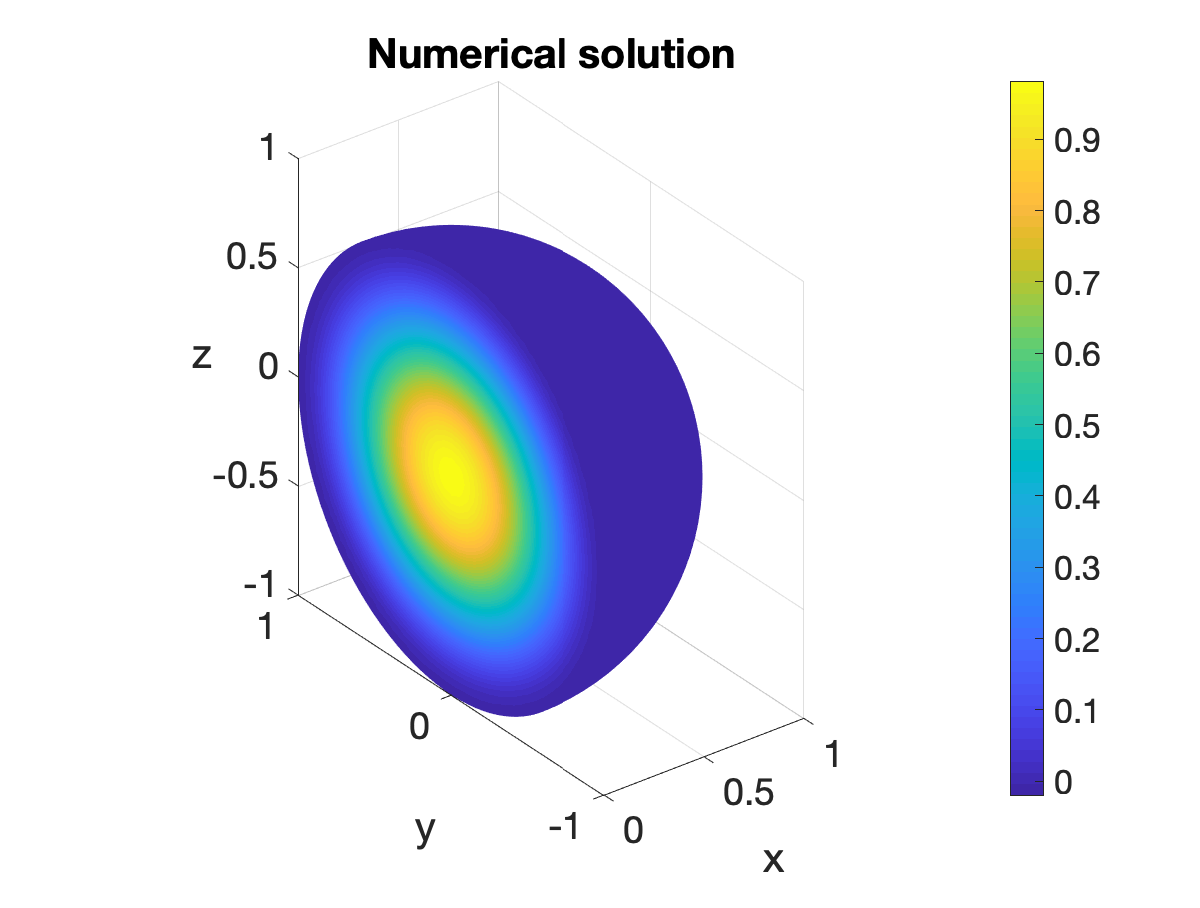
\includegraphics[scale=0.5]{laplace3dsphere_Nx41.eps}
\end{center}
\caption{Laplace equation \eqref{experiment_laplace_equation_3d_sphere} on the unit sphere $\Omega$ in 3D: numerical solution obtained on the finest mesh for $i=4$ with $N= 40381$ nodes.}
\label{fig:laplace_3d_numsol_sphere}
\end{figure} 

\section{Numerical examples for bulk-surface problems}

\subsection{Elliptic bulk-surface problem on the sphere}
\label{sec:example_elliptic_bs_sphere}
We numerically solve the following elliptic bulk-surface problem,  found in \cite{elliott2013finite}, on the unit sphere $\Omega$ in 3D:
\begin{equation}
\label{experiment_bs_3d_sphere}
\begin{cases}
-&\Delta u + u = xyz \qquad \text{in}\ \Omega\\
-&\Delta_\Gamma v + v +\nabla u\cdot\boldn = 29xyz \qquad \text{on}\ \partial \Omega\\
&\nabla u \cdot \boldn = -u + 2v   \qquad \text{on}\ \partial \Omega
\end{cases}
\end{equation}
whose exact solution is given by
\begin{align*}
&u(x,y,z) = xyz, \qquad (x,y,z) \in \Omega;\\
&v(x,y,z) = 2xyz, \qquad (x,y,z) \in \partial\Omega.
\end{align*}
We consider the same sequence of four meshes $\Omega_i$, $i=1,2,3,4$ of Experiment \ref{sec:laplace_sphere}.  The surface meshes are induced by the corresponding bulk mesh, i.e. $\Gamma_i = \partial \Omega_i$, $i=1,\dots,4$. On each mesh we solve the discrete problem,  we compute the error in $L^2(\Omega)\times L^2(\Gamma)$ norm and the respective convergence rate. As shown in Table \ref{tab:bs_3d_convergence_sphere}, the convergence in $L^2(\Omega)\times L^2(\Gamma)$ norm is optimal, i.e. quadratic. The numerical solution obtained on the finest mesh is plotted in Fig.  \ref{fig:bs_3d_numsol_sphere}.

\begin{table}[H]
\caption{Elliptic bulk-surface problem \eqref{experiment_bs_3d_sphere} on the unit sphere $\Omega$ in 3D. The VEM implemented in VEMLAB shows optimal quadratic convergence in $L^2(\Omega) \times L^2(\Gamma)$ norm. Times required for the solution of the linear system are shown.}
\begin{center}
\begin{tabular}{c | c | c | c | c | c}
$i$ & $N$ & $h$ & $L^2(\Omega)\times L^2(\Gamma)$ error & $L^2(\Omega)\times L^2(\Gamma)$ rate & Time (s)\\
\hline
1 & 111 & 0.6928 &   2.1985e-01 &  -   & 0.002159\\
2 & 799 & 0.3464 & 3.8387e-02 & 2.5178    & 0.015645\\
3 & 5749 & 0.1732 & 8.5674e-03 & 2.1637  & 0.197641  \\
4 & 40381 & 0.0866 &  1.9884e-03 & 2.1072 & 5.994934
\end{tabular}
\end{center}
\label{tab:bs_3d_convergence_sphere}
\end{table}

\begin{figure}[H]
\begin{center}
\hspace*{-10mm}
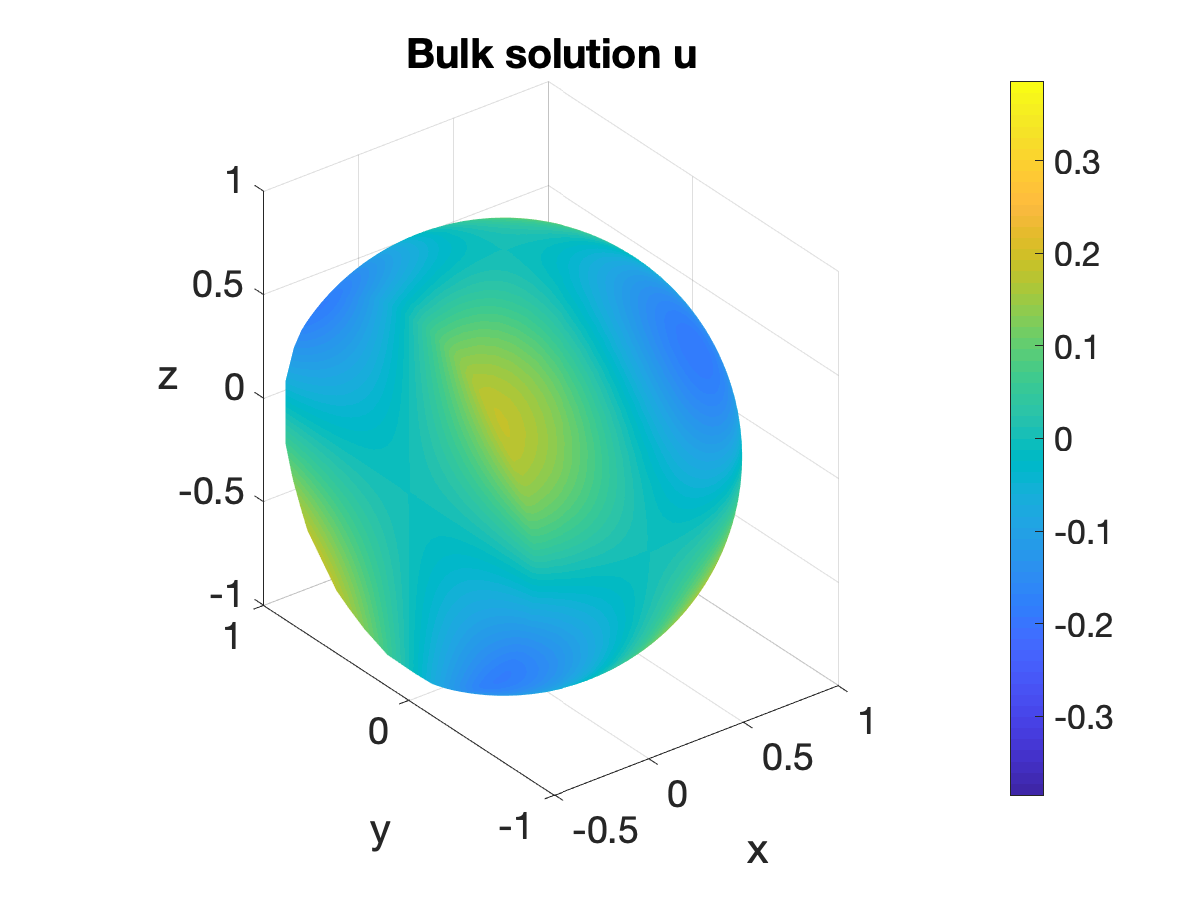
\includegraphics[scale=0.4]{bs_3d_sphere_nx41_u.eps}
\hspace*{-5mm}
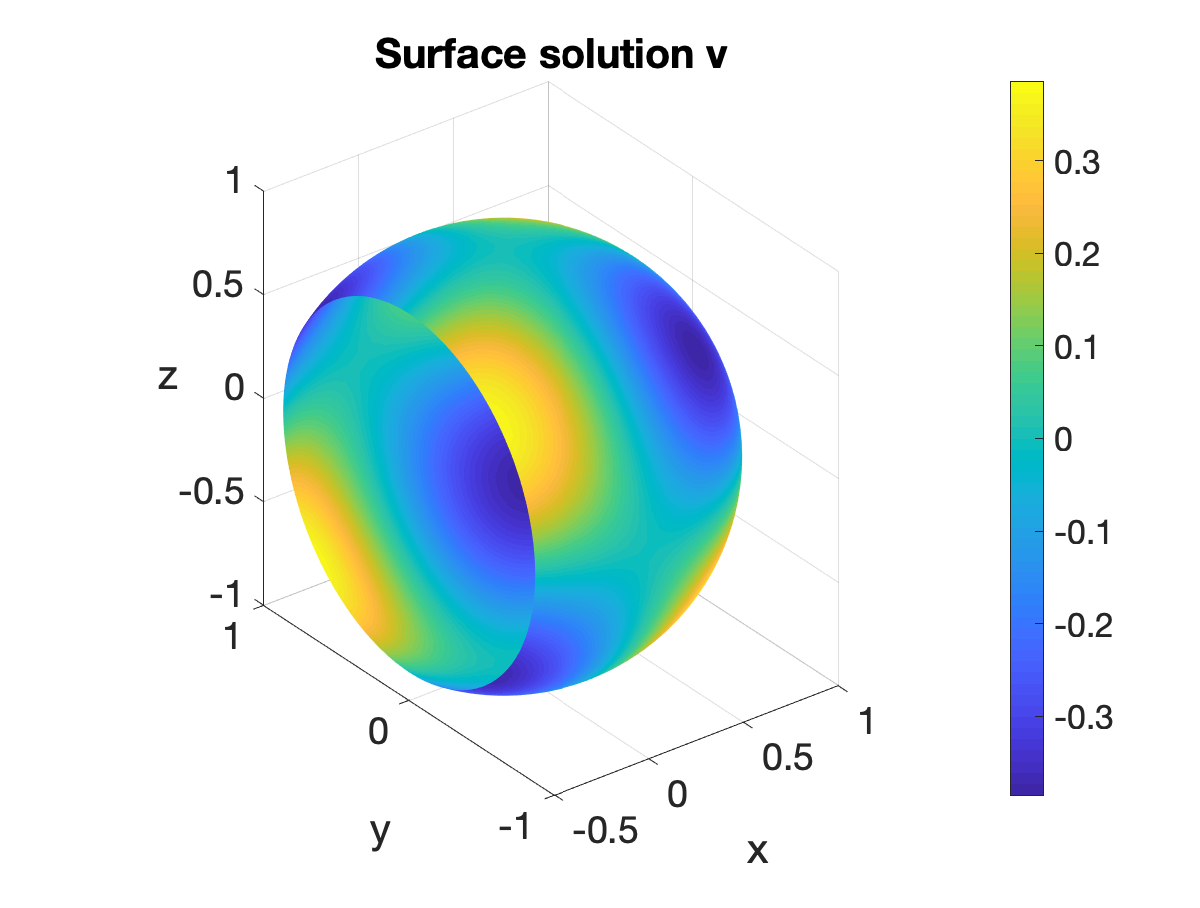
\includegraphics[scale=0.4]{bs_3d_sphere_nx41_v.eps}
\end{center}
\caption{Elliptic bulk-surface  problem \eqref{experiment_bs_3d_sphere} on the unit sphere $\Omega$ in 3D: numerical solution obtained on the finest mesh for $i=4$ with $N= 40381$ nodes. Left: bulk component $u$. Right: surface component $v$.}
\label{fig:bs_3d_numsol_sphere}
\end{figure} 

\subsection{Parabolic bulk-surface problem on the sphere}
We numerically solve the following parabolic bulk-surface problem,  found in \cite{frittelli2021bulk}, on the unit sphere $\Omega$ in 3D:
\begin{equation}
\label{experiment_bs_3d_sphere_parabolic}
\begin{cases}
&\dot{u} -\Delta u  = xyze^t \qquad  \text{in}\ \Omega \times [0,T];\\
&\dot{v} -\Delta_\Gamma v +\nabla u\cdot\boldn = 16xyze^t \qquad \text{on}\ \partial \Omega \times [0,T];\\
&\nabla u \cdot \boldn = 3xyze^t  \qquad \text{on}\ \partial \Omega \times [0,T],
\end{cases}
\end{equation}
for final time $T=1$, whose exact solution is given by
\begin{align*}
&u(x,y,z,t) = xyze^t, \qquad (x,y,z,t) \in \Omega \times [0,T];\\
&v(x,y,z,t) = 2xyze^t, \qquad (x,y,z,t) \in \partial\Omega \times [0,T].
\end{align*}
We consider the same sequence of four meshes $\Omega_i$, $i=1,2,3,4$ of Experiment \ref{sec:example_elliptic_bs_sphere}.  Correspondingly, we choose timesteps $\tau_i = 2^{1-i}$,  $i=1,2,3,4$. On each mesh we solve the discrete problem,  we compute the error in $L^2(\Omega)\times L^2(\Gamma)$ norm at the final time $T=1$ and the respective convergence rate. As shown in Table \ref{tab:bs_3d_convergence_sphere_parabolic}, the convergence in $L^2(\Omega)\times L^2(\Gamma)$ norm is optimal, i.e. quadratic in space and linear in time. The numerical solution at the final time obtained on the finest mesh is plotted in Fig.  \ref{fig:bs_3d_numsol_sphere_parabolic}.

\begin{table}[H]
\caption{Parabolic bulk-surface problem \eqref{experiment_bs_3d_sphere_parabolic} on the unit sphere $\Omega$ in 3D. The VEM implemented in VEMLAB shows optimal quadratic convergence in $L^2(\Omega) \times L^2(\Gamma)$ norm. Times required for the time integration are shown.}
\begin{center}
\begin{tabular}{c | c | c | c | c | c | c}
$i$ & $N$ & $h$ & $\tau$ & $L^2(\Omega)\times L^2(\Gamma)$ error & $L^2(\Omega)\times L^2(\Gamma)$ rate & Time (s)\\
\hline
1 & 111 & 0.6928 &   1 & 1.2074 &  -   & 0.002417\\
2 & 799 & 0.3464 & 2.5e-1 & 4.3481e-01 & 1.4734    & 0.038881\\
3 & 5749 & 0.1732 & 6.25e-2 & 1.2110e-01 & 1.8442  & 2.134601  \\
4 & 40381 & 0.0866 &  1.5625e-2 & 3.0881e-02 & 1.9714 & 287.345570
\end{tabular}
\end{center}
\label{tab:bs_3d_convergence_sphere_parabolic}
\end{table}

\begin{figure}[H]
\begin{center}
\hspace*{-10mm}
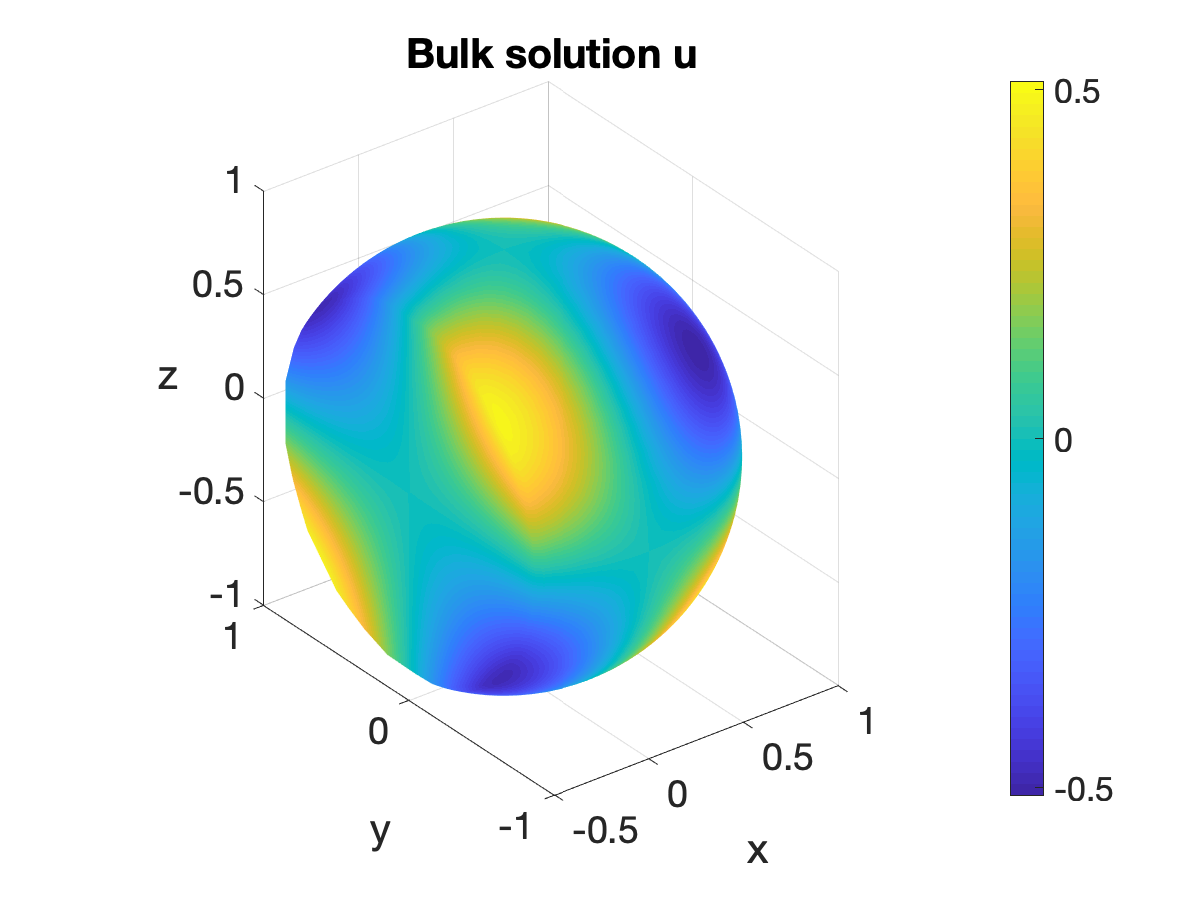
\includegraphics[scale=0.4]{bs_3d_sphere_nx41_parabolic_u.eps}
\hspace*{-5mm}
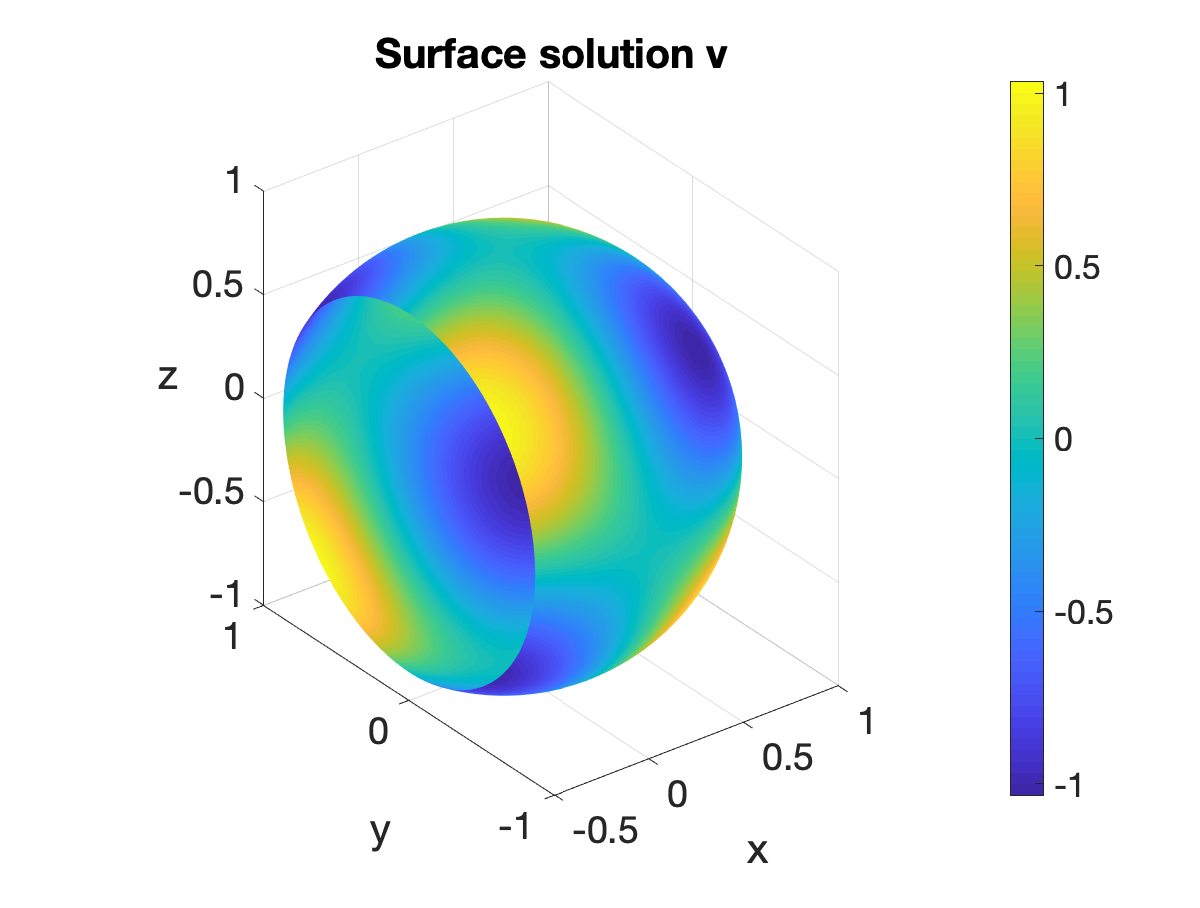
\includegraphics[scale=0.4]{bs_3d_sphere_nx41_parabolic_v.eps}
\end{center}
\caption{Parabolic bulk-surface  problem \eqref{experiment_bs_3d_sphere_parabolic} on the unit sphere $\Omega$ in 3D: numerical solution obtained on the finest mesh for $i=4$ with $N= 40381$ nodes and timestep $\tau = 1.5625e-2$. Left: bulk component $u$. Right: surface component $v$.}
\label{fig:bs_3d_numsol_sphere_parabolic}
\end{figure} 
 
\bibliographystyle{plain}
\bibliography{bibliography}
 

\end{document}